\documentclass[problems]{esg8022pset} 
\usepackage{amsmath}
\usepackage{amssymb}
\usepackage{enumerate}
\usepackage{graphicx}
\usepackage{hyperref}
\usepackage{mathtools}
\usepackage[per-mode=symbol]{siunitx} %If this line is giving you trouble, try replacing per-mode with per
%use inter-unit-separator={}\cdot{} ?
\providecommand{\uvec}[1]{{\hat{\bf{#1}}}}
\usepackage{pgf,tikz}
\usetikzlibrary{arrows}
\usepackage{wasysym}
\usepackage{subfig}
\makeatletter
\newcommand{\interitemtext}[1]{%
  \begin{list}{}
   {\itemindent=0mm\labelsep=0mm
   \labelwidth=0mm\leftmargin=0mm
   \addtolength{\leftmargin}{-\@totalleftmargin}}
    \item #1
  \end{list}
}
\makeatother
\renewcommand{\d}{\,d}
\providecommand{\norm}[1]{\lVert#1\rVert}

\newcommand{\Kgrad}{\left(\hat{x} \frac{\partial}{\partial x} + \hat{y} \frac{\partial}{\partial y} + \hat{z} \frac{\partial}{\partial z}\right)}
\newcommand{\Kdiv}[6]{{#4}\left(\frac{\partial {#1}}{\partial x} {#5} \frac{\partial {#2}}{\partial y} {#6}\frac{\partial #3}{\partial z} \right)}
\newcommand{\KKdiv}[6]{{#4}\left(\frac{\partial}{\partial x}{#1} {#5} \frac{\partial}{\partial y}{#2} {#6}\frac{\partial}{\partial z}{#3} \right)}
\newcommand{\dx}{\frac{\partial}{\partial x}}
\newcommand{\dy}{\frac{\partial}{\partial y}}
\newcommand{\dz}{\frac{\partial}{\partial z}}
\newcommand{\dtheta}{\frac{\partial}{\partial \theta}}
\newcommand{\dr}{\frac{\partial}{\partial r}}

\AtBeginDocument{%
  % Appologies to any future editor on the inconsistencies in TeX code and the unnecessary braces.  I'm aggregating previously typeset problems, and didn't think it worth my time to improve the quality of TeX code in ways that won't make any difference to the typeset material. -Jason Gross (jgross@mit.edu)
}%
\classname{Physics 8.022} \semester{Spring 2011} 
\problemsetnumber{10}
\date{\today }
\duedate{Wednesday, April 27th, 10 pm}
\readingassignment{}
\problemsettitle{RLC circuits, AC circuits}
\begin{document}
\section{Problem \thesection: Purcell 7.17}
\begin{figure}[H]
    \centering
    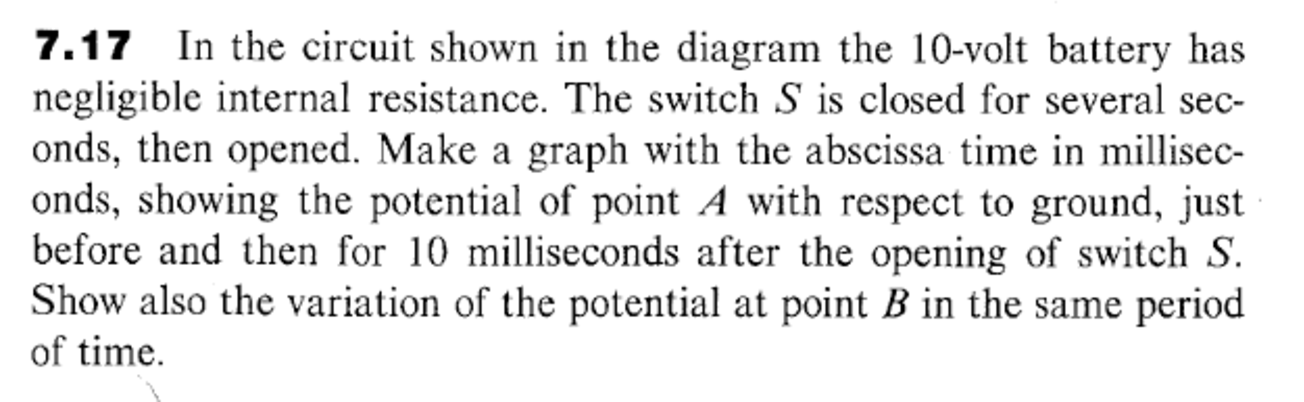
\includegraphics[width = 10cm]{pu717}
    \caption{Purcell 7.17}
  \end{figure}

  \begin{figure}[H]
    \centering
    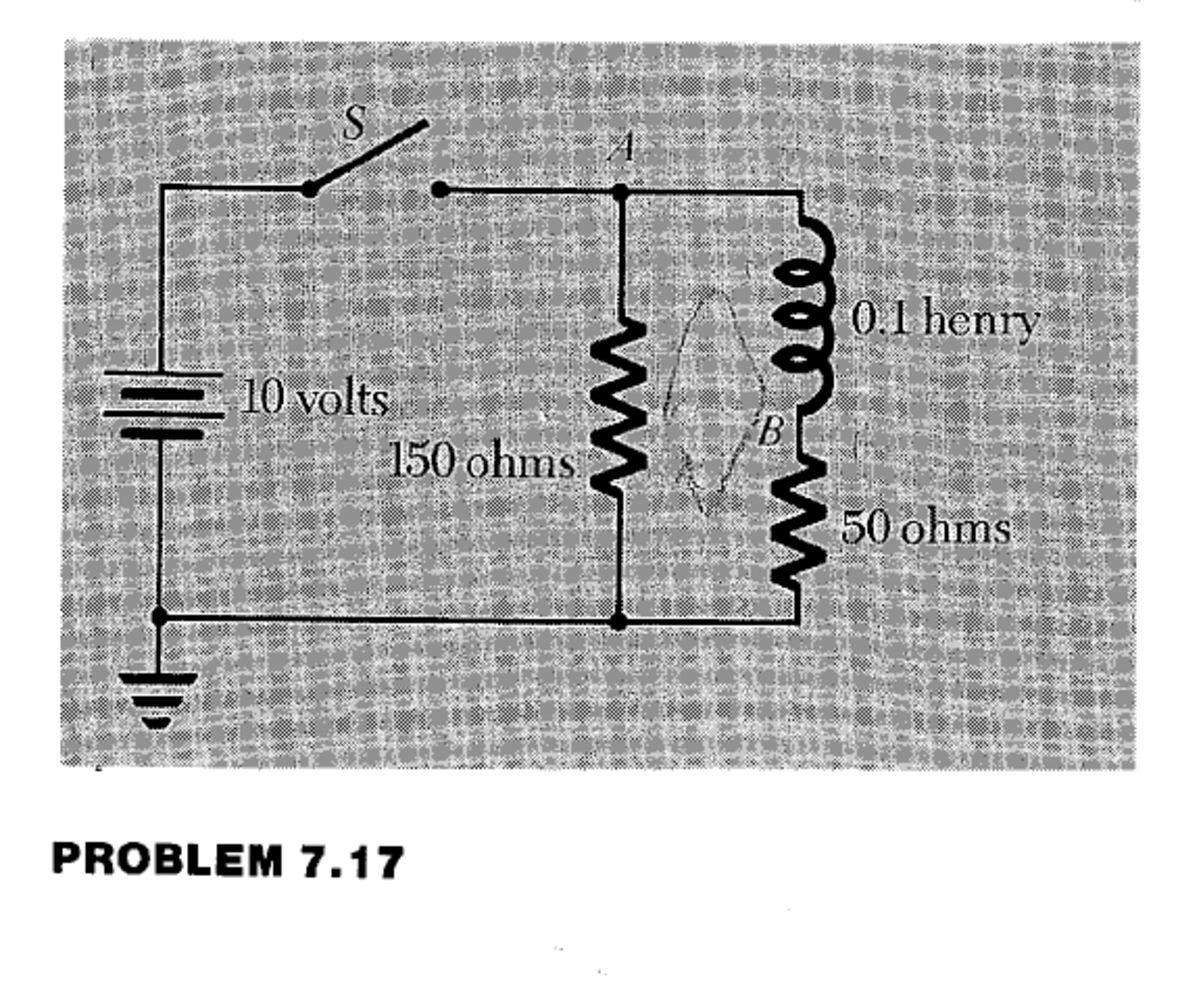
\includegraphics[width = 10cm]{figpu717}
    \caption{Figure Purcell 7.17}
  \end{figure}

 Extra question --- By grounding this circuit, we make the switch
safer to operate. Describe why a large spark jumps across the switch
when it is not grounded, and why the spark does not happen when it is
grounded.
\section{Problem \thesection: Purcell 8.4}
\begin{figure}[H]
    \centering
    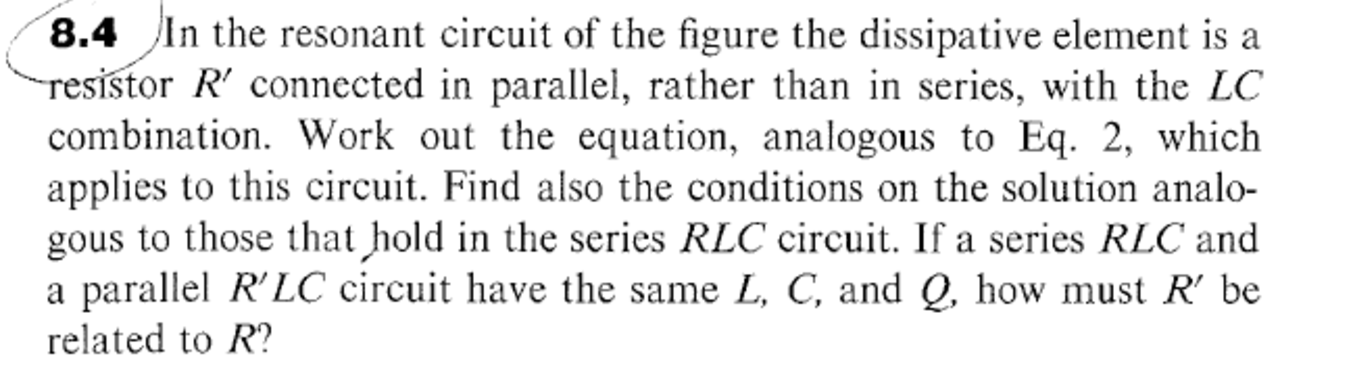
\includegraphics[width = 10cm]{pu804}
    \caption{Purcell 8.04}
  \end{figure}

  \begin{figure}[H]
    \centering
    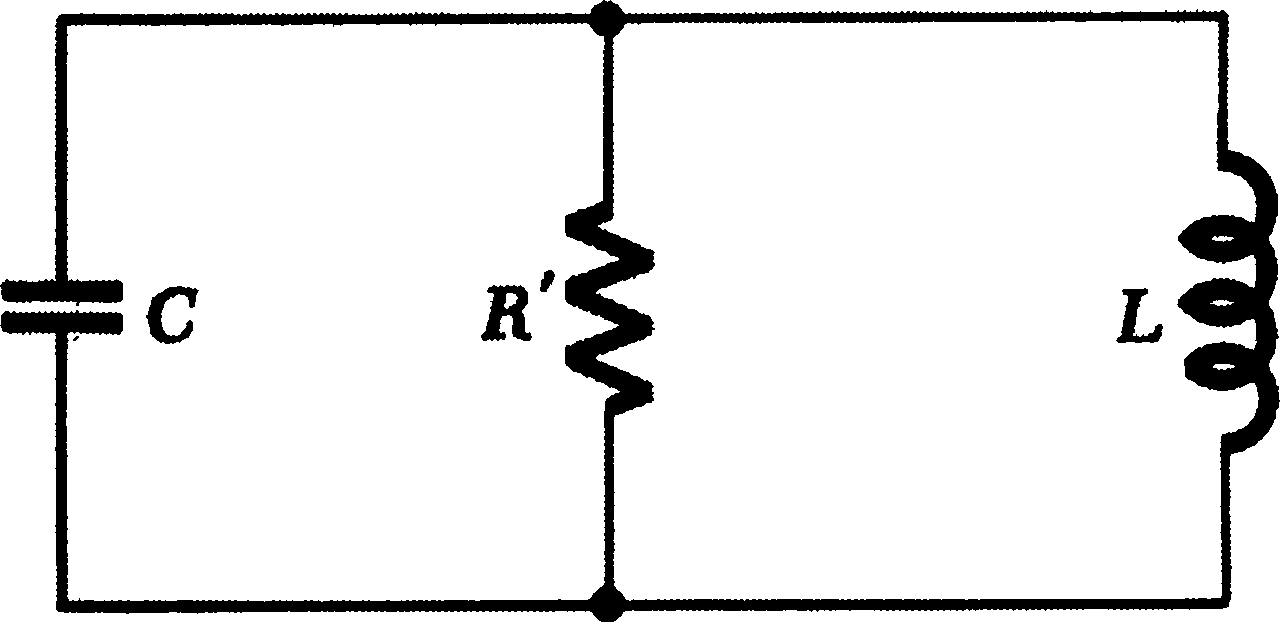
\includegraphics[width = 10cm]{figpu804}
    \caption{Purcell 8.04}
  \end{figure}

\section{Problem \thesection: Purcell 8.7}
 A resonant cavity of the form illustrated is an essential part of many microwave oscillators. It can be regarded as a simple $LC$ circuit. The inductance is that of a toroid with one turn. Find an expression for the resonant frequency of this circuit and show by a sketch the configuration of the magnetic and electric fields.
 Hint: the capacitor is composed by the upper and lower disks
 \begin{figure}[H]
    \centering
    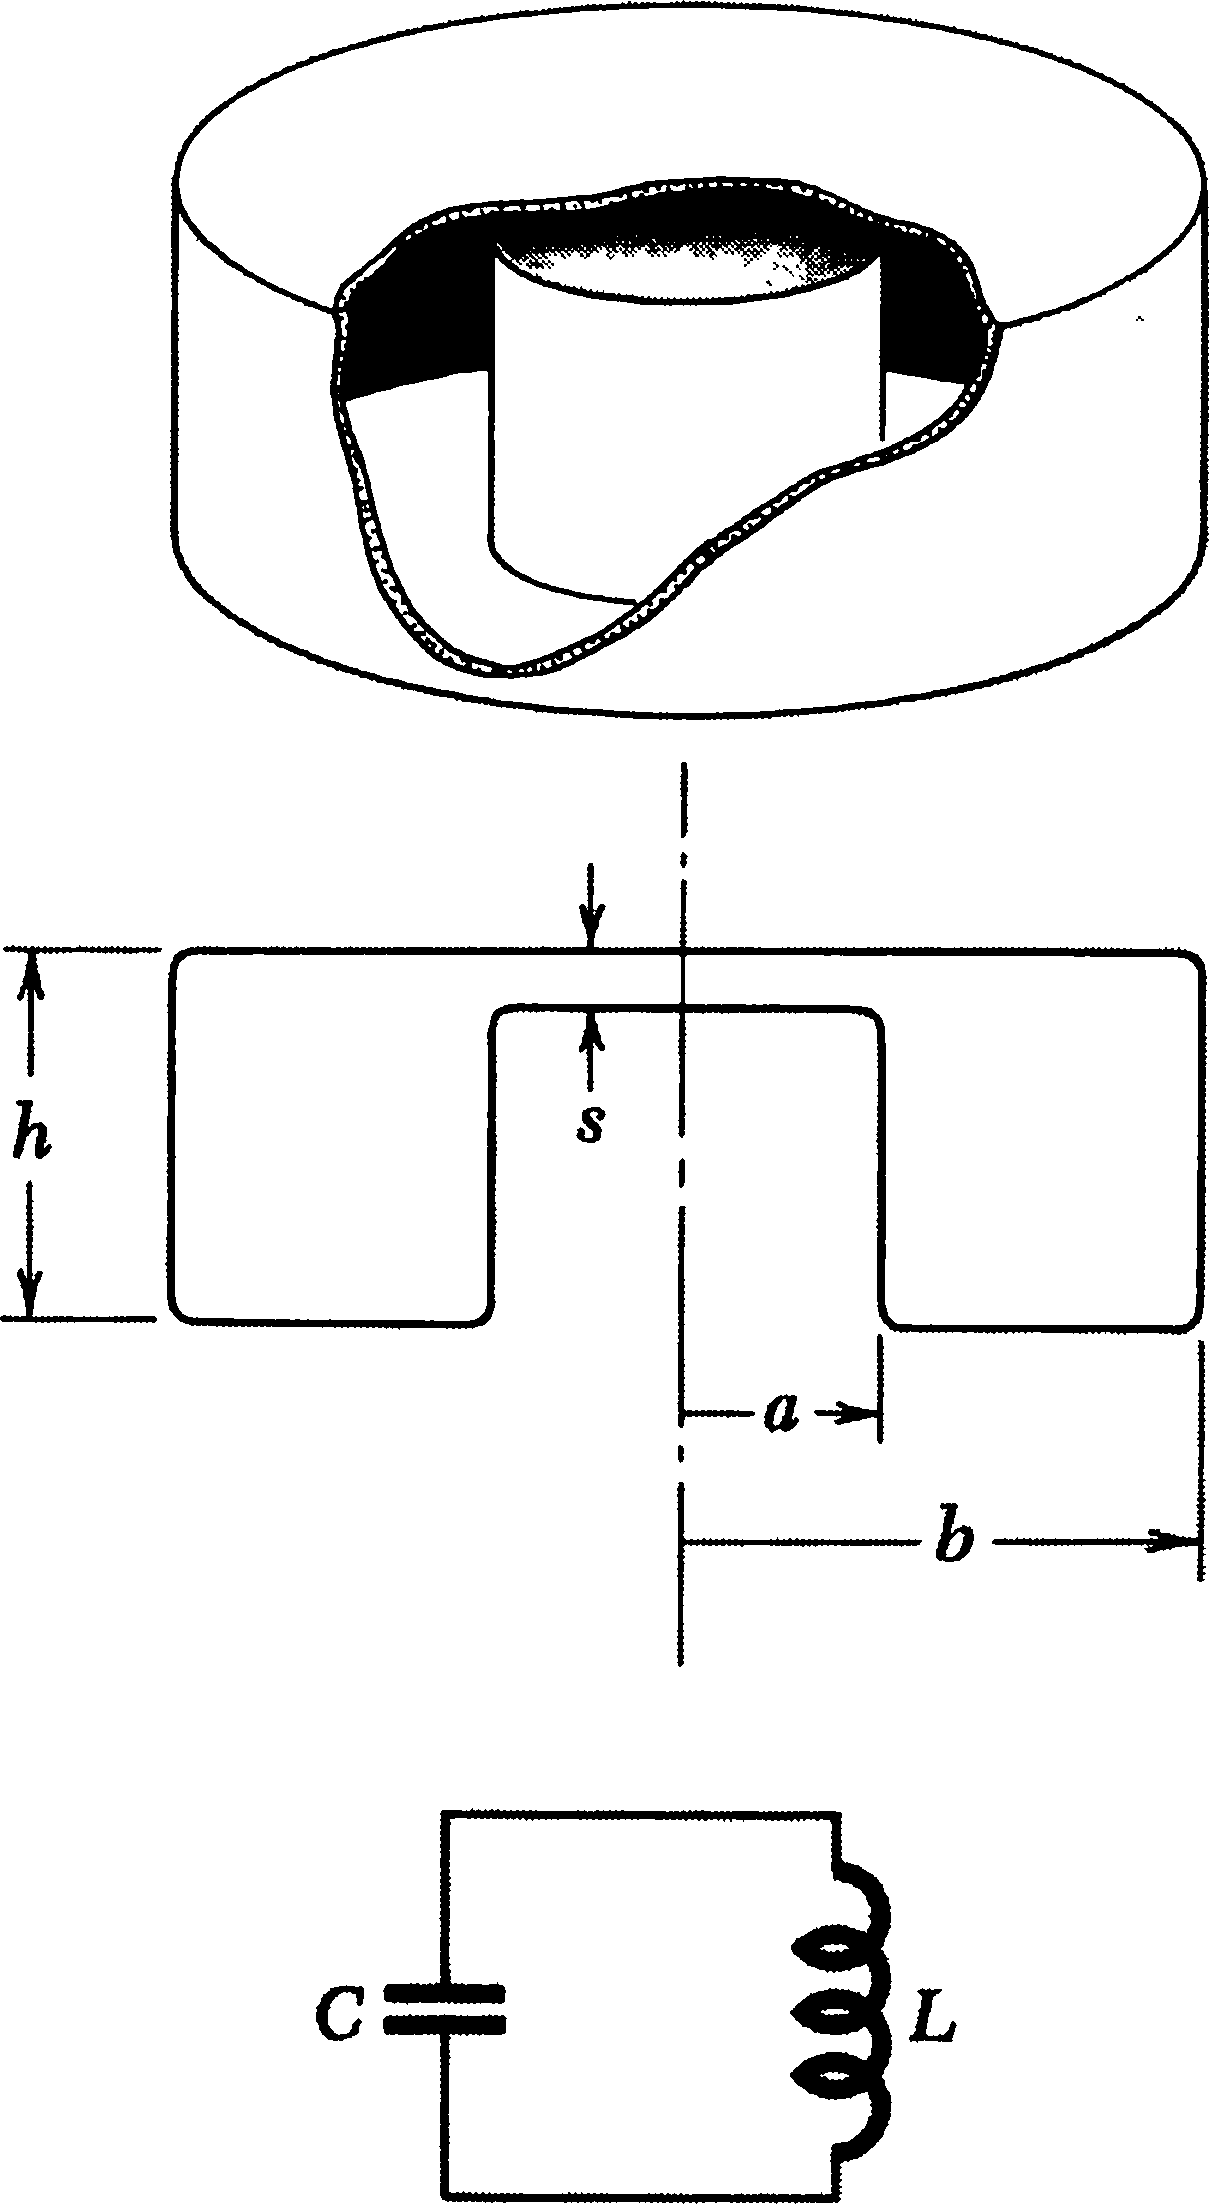
\includegraphics[width = 4cm]{pu807}
    \caption{Purcell 8.7}
    \label{fig:cavity2}
  \end{figure}

\section{Problem \thesection: Purcell 8.9}
\begin{figure}[H]
    \centering
    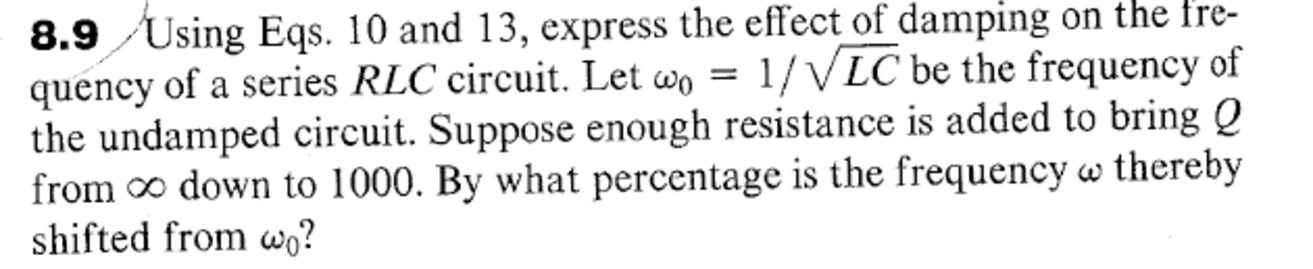
\includegraphics[width = 10cm]{pu809}
    \caption{Purcell 8.09}
  \end{figure}

  \begin{figure}[H]
    \centering
    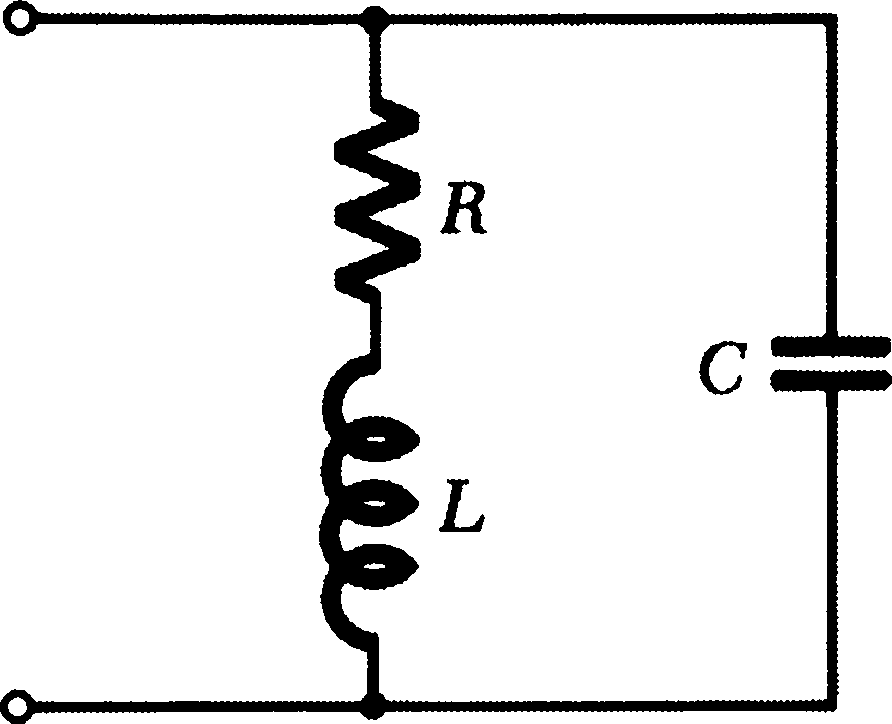
\includegraphics[width = 10cm]{figpu809}
    \caption{Purcell 8.09}
  \end{figure}
\section{Problem \thesection: Purcell 8.12}

\begin{figure}[H]
    \centering
    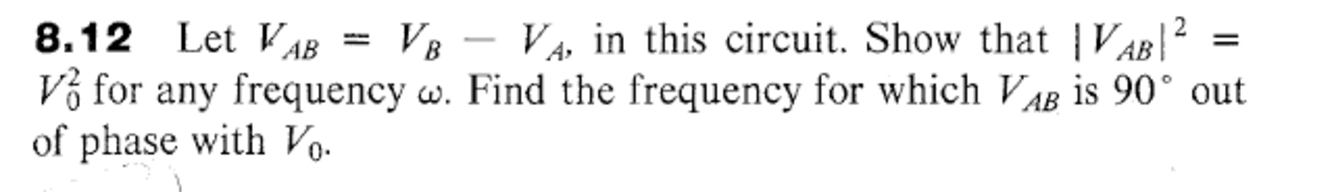
\includegraphics[width = 10cm]{pu812}
    \caption{Purcell 8.12}
  \end{figure}

  \begin{figure}[H]
    \centering
    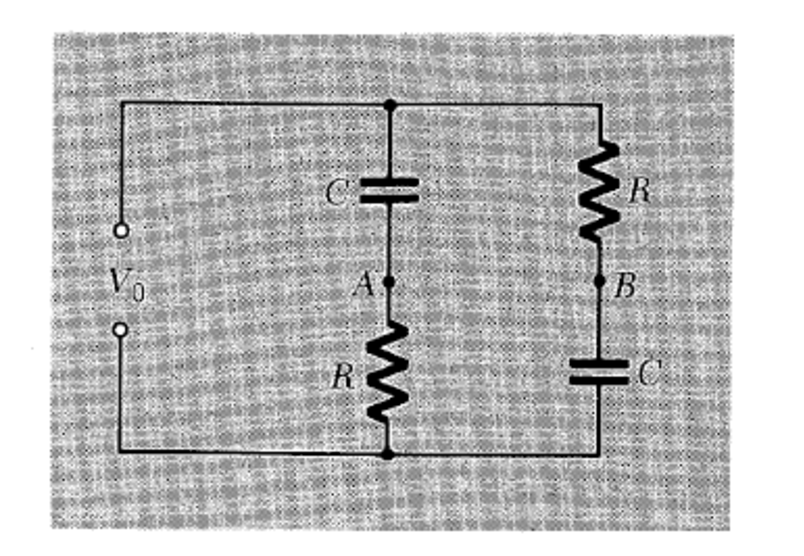
\includegraphics[width = 10cm]{figpu812}
    \caption{Purcell 8.12}
  \end{figure}
\section{Problem \thesection: Purcell 8.16}


\begin{figure}[H]
    \centering
    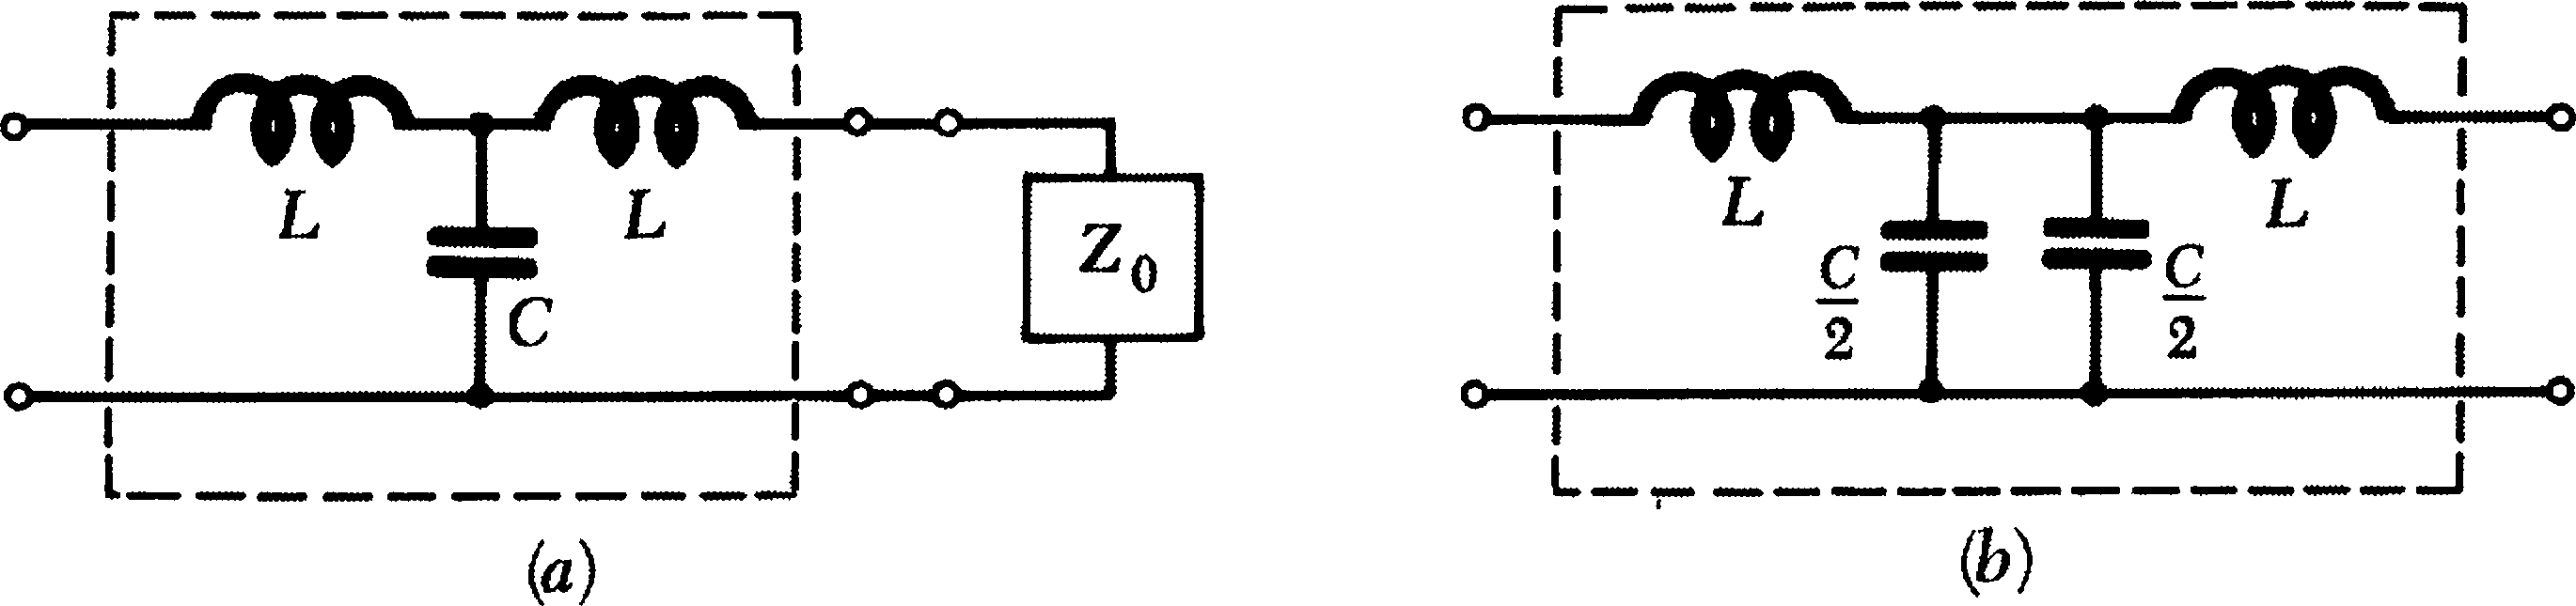
\includegraphics[width = 10cm]{pu816}
    \caption{Purcell 8.16}}
    \label{pu816}
  \end{figure}

An impedance $Z_o$ is to be connected to the terminals on the right. For given frequency $\omega$ find the value which $Z_o$ must have if the resulting impedance between the left terminals is $Z_o$. The required $Z_o$ is a pure resistance $R_o$ provided $\omega^2<2/LC$. What is $Z_o$ in the special case $\omega = \sqrt{2/LC}$?


\section{Problem \thesection: Optional Purcell 8.10}
\begin{figure}[H]
    \centering
    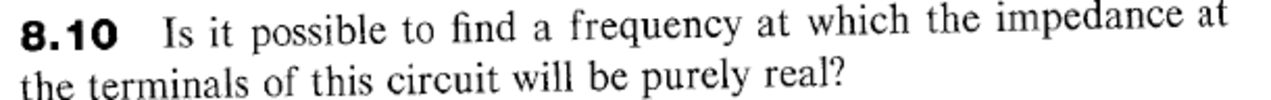
\includegraphics[width = 10cm]{pu810}
    \caption{Purcell 8.10}
  \end{figure}

  \begin{figure}[H]
    \centering
    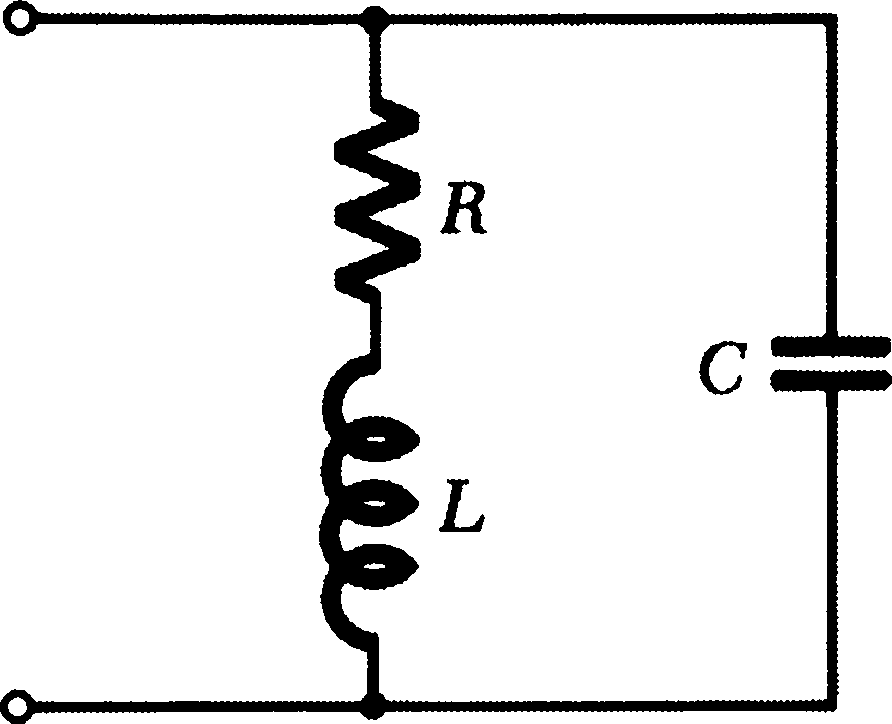
\includegraphics[width = 10cm]{figpu810}
    \caption{Purcell 8.10}
  \end{figure}
\section{Problem \thesection:  Optional Purcell 8.13}

\begin{figure}[H]
    \centering
    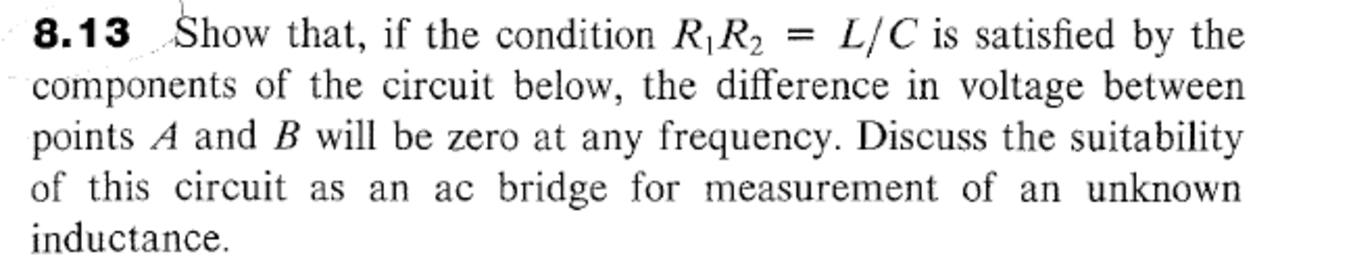
\includegraphics[width = 10cm]{pu813}
    \caption{Purcell 8.13}
  \end{figure}

  \begin{figure}[H]
    \centering
    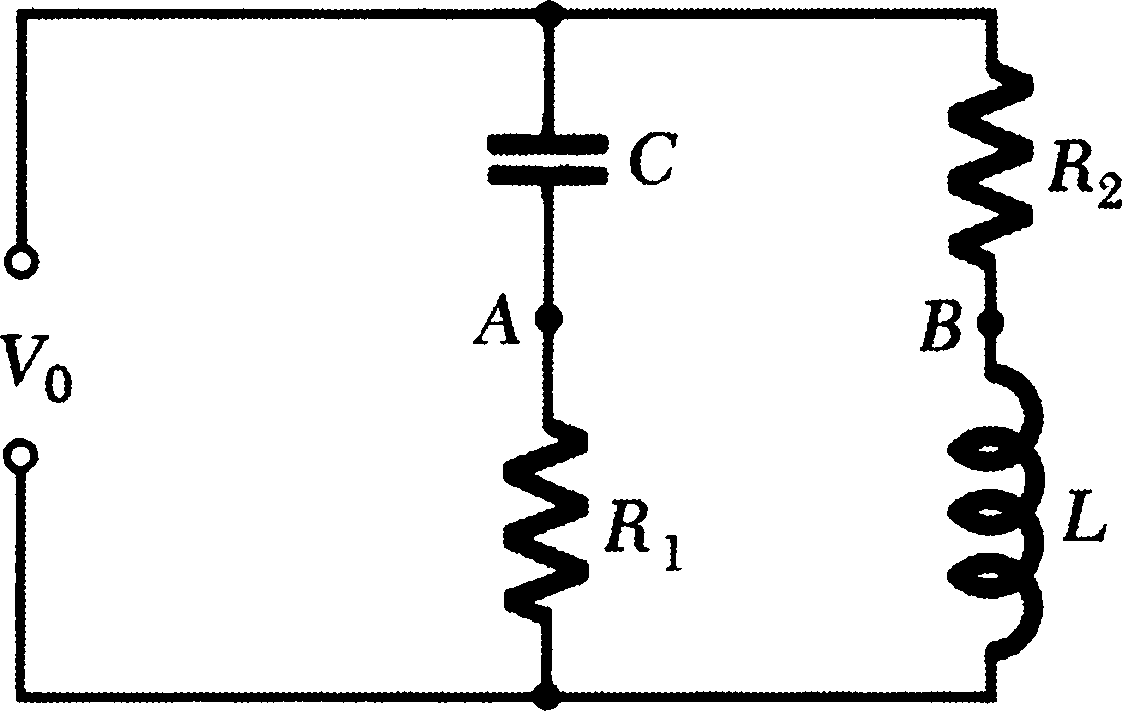
\includegraphics[width = 10cm]{figpu813}
    \caption{Purcell 8.13}
  \end{figure}

\section{Problem \thesection: Optional Purcell 8.14}
\begin{figure}[H]
    \centering
    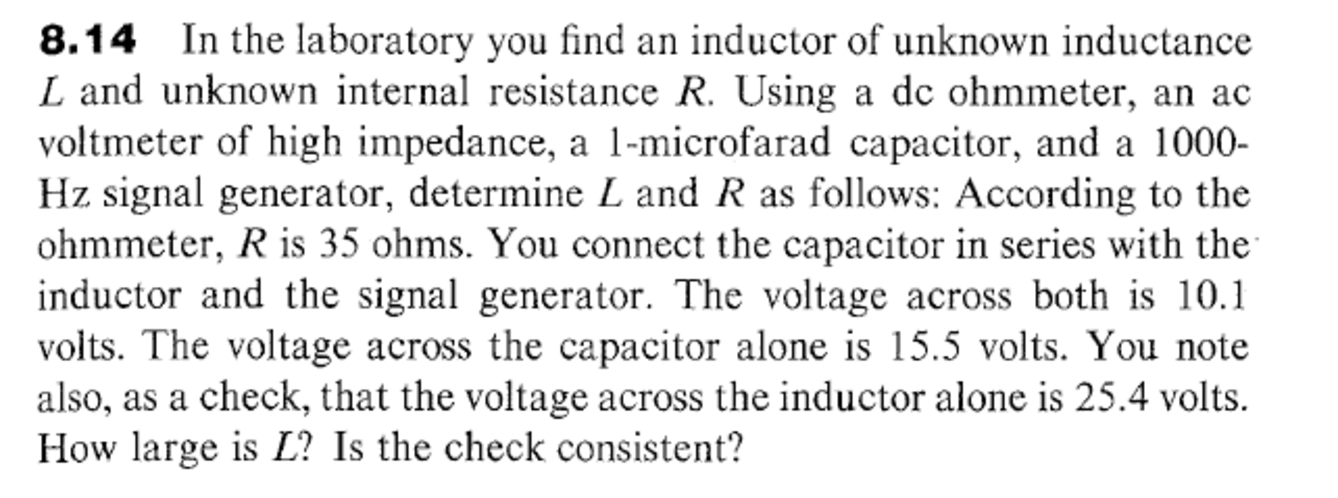
\includegraphics[width = 10cm]{pu814}
    \caption{Purcell 8.14}
  \end{figure}


\end{document}
